\chapter{Entwicklung von Erweiterungen} \label{extending}
\addthumb{Entwicklung von Erweiterungen}{\huge{\textbf{\thechapter.}}}{white}{haw_rot} 

Das Java Medical Imaging Toolkit bietet sowohl dem Enwickler, als auch dem Anwender Spielraum, die Anwendung zu erweitern. Dieses Kapitel beschreibt die Entwicklung verschiedener Plug-ins in zwei- und dreidimensionalem Raum. Zusätzlich zeigt der Entwurf eines neuen Moduls und eine Implementierung eines Werkzeugs wie die Basisfunktionen von jMediKit erweitert werden.

\FloatBarrier
\section{Entwicklung von Plug-ins}

Die Entwicklung von Plug-ins ermöglicht eine Funktionserweiterung der Anwendung, ohne einen neuen Buildprozess. Bei Programmstart wird der in der Anwendung angegebene Plug-in-Ordner nach allen verfügbaren Erweiterungen durchsucht und eingebunden. Damit Plug-ins vom Programm korrekt gefunden werden können, müssen diverse Konventionen bei der Entwicklung beachtet werden, die im nächsten Abschnitt erläutet werden.

\FloatBarrier
\subsection{Konventionen}
Damit der Importvorgang der Plug-ins ohne Komplikationen verläuft, ist die Anwendung auf die Konsistenz der Plug-ins angwiesen. Die folgenden Konventionen bestimmen diese Konsistenz.

\begin{itemize}
\item \textbf{Generalisierung}\\
Die Basisklasse eines Plug-ins ist entweder \textit{APlugIn2D} oder \textit{APlugIn3D} und muss diese erweitern. 
\item \textbf{Klassenname}\\
Der Name der Klasse des Plug-ins, die von \textit{APlugIn2D} oder \textit{APlugIn3D} erbt, muss mit \textit{zwei Unterstrichen} beginnen. Zusätzlich muss das erste Zeichen ein Buchstabe oder eine Ziffer sein. Listing \ref{regexp} zeigt den regulären Ausdruck zur Beurteilung gültiger Namen. Korrekt sind zum Beispiel \textit{\_\_Test} oder \textit{\_\_3DTest\_Plug\_in}. Ungültig ist beispielsweise \textit{\_Test} oder \textit{\_\_\_TestPlugIn}.
Da ein Plug-in in Beziehung zu anderen Klassen oder Paketen stehen kann, die entweder selbst implementiert oder von Bibliotheken zur Verfügung gestellt werden, wird so die Hauptklasse der Erweiterung kenntlich gemacht.
\item \textbf{Ordnername}\\
Der Ordner, in dem ein Plug-in enthalten ist, muss den identischen Namen wie die Hauptklasse des Plug-ins haben. Ist dieser Name \textit{\_\_Test}, muss der \textit{Wurzelordner} der die Erweiterung enthält ebenfalls \textit{\_\_Test} heißen.
\item \textbf{Ordnerstruktur}\\
Wenn Plug-ins mit Hilfe der Eclipse-Entwicklungsumgebung entwickelt werden, entspricht der Output-Ordner mit den \textit{.class-Dateien} eines Eclipse-Projekts der korrekten Struktur. Ist die Hauptklasse nicht in einem Package organisiert, liegt die Plug-in-Klasse direkt im Plug-in-Ordner und hätte die Struktur \textit{/plugins/\_\_Test/\_\_Test.class}. Erfolgt die Entwicklung mit Packages ist die Struktur \textit{/plugins/\_\_Test/de/korb/\_\_Test.class} wenn die Klasse \_\_Test im Package \textit{de.korb} liegt. \textit{/plugins} ist der Ordner, der die einzelnen Plug-ins enthält. Dieser muss in den Einstellungen der Anwendung spezifiziert werden. Das bedeutet, dass jMediKit alle Plug-ins in \textit{/plugins} findet, wenn die Ordner mit doppeltem Unterstrich beginnen und eine \textit{.class}-Datei mit identischen Namen beinhalten, die APlugIn2D oder APlugIn3D generalisieren. Abbildung \ref{filesystemplugin} zeigt die Ordnerstruktur zweier Plug-ins. \_\_PlugInA ist ohne, während \_\_PlugInB mit Packages organisiert wird. \_\_PlugInB definiert zusätzlich eine eigenen Bibliotheksklasse. Wird der Ordner \textit{plugins} in den Einstellungen angegeben, werden bei Programmstart die beiden Plug-ins initialisiert und können verwendet werden. Nach einer neuen Belegung der Einstellungen, muss die Anwendung neu gestartet werden.
\end{itemize}

\lstset{
language=sh,
caption={Der reguläre Ausdruck gültiger Klassennamen},
label=regexp,
xleftmargin=1em,
xrightmargin=1em,
numbers=left,
backgroundcolor=\color{lgrey},
}  
\begin{figure}[htbp]
\begin{lstlisting}[frame=leftline]
^_[A-Za-z0-9].*
\end{lstlisting}
\end{figure}

\tikzstyle{every node}=[draw=black,thick,anchor=west]
%\tikzstyle{selected}=[draw=red,fill=red!30]
\tikzstyle{optional}=[dashed,fill=gray!50]
\begin{figure}[htbp]
\centering
\caption{Beispiel der Ordnerstruktur zwei verschiedener Plug-ins}
\label{filesystemplugin}
\begin{tikzpicture}[%
 grow via three points={one child at (0.5,-0.7) and
  two children at (0.5,-0.7) and (0.5,-1.4)},
  edge from parent path={(\tikzparentnode.south) |- (\tikzchildnode.west)}]
  \node {plugins}
    child[missing]{}
    child{ node{\_\_PlugInA}
      child[missing]{}
      child { node{\_\_PlugInA.class}}
    }
    child[missing]{}
    child[missing]{}
    child[missing]{}
    child { node{\_\_PlugInB}
      child[missing]{}
      child { node{de}
        child{ node{core}
          child{node{\_\_PlugInB.class}} 
        }
        child[missing]{}
        child{ node{lib}
          child{node{Library.class}} 
        }
      }
    };		
\end{tikzpicture}
\end{figure}


    	%child { node{\_\_PlugInA.class}}
    	
    	%child { node{\_\_PlugInB}
    	   %child { node{de}
    	   %  child{ node{core}
    	   %    child{node{\_\_PlugInB.class}} 
    	   %  }
    	   %  child{ node{lib}
    	   %    child{node{Library.class}} 
    	   %  }
    	   %}
    	%}
\FloatBarrier
\subsection{Die Klassenstruktur eines Plug-ins}

Das Java Medical Imaging Toolkit stellt zwei Typen von Plug-ins bereit. Der Anwender kann mit einer Erweiterung von APlugIn2D entweder im zweidimensionalen oder mit APlugIn3D im dreidimensionalen Raum arbeiten. Unabhängig vom Plug-in-Typ müssen zwei abstrakte Methoden der jeweiligen Basisklasse implementiert werden.

\begin{itemize}
\item \textbf{options}\\
Die Methode \textit{options} wird \textit{einmalig} \textit{vor} der Ausführung des Plug-ins aufgerufen. Hier können wahlweise Parameter gesetzt werden, die für weitere Berechnungen benötigt werden.
\item \textbf{process}\\
Das Kernelement eines Plug-ins stellt \textit{process} dar. Als Parameter ist entweder das aktuell gewählte Bild im ImageView oder im Fall eines 3D-Plug-ins der Bildstapel als Parameter der Methode enthalten. Beim Rückgabewert muss beachtet werden, dass die Bildanzahl mit der im Parameter übereinstimmt, da sonst weitere Berechnungen, wie zum Beispiel die Ebenenrekonstruktionen, nicht korrekt ausgeführt werden können.

\end{itemize}

In Listing \ref{zweid} ist die Basisdefinition eines zweidimensionalen Plug-ins dargestellt. Es werden die abstrakten Methoden \textit{process} und \textit{options} implementiert. Mit dem Parameter \textit{img} in \textit{process} können die Pixelwerte manipuliert werden. Das Rückgabebild wird anschließend im ImageView an Stelle des entsprechenden Index angezeigt.

\lstset{
language=Java,
caption={Definition des konkreten 2D-Plug-ins \_\_2dPlugIn.java},
label=zweid,
xleftmargin=1em,
xrightmargin=1em,
numbers=left,
backgroundcolor=\color{lgrey},
}  
\begin{figure}[htbp]
\begin{lstlisting}[frame=leftline]
public class __2dPlugIn extends APlugIn2D{
 @Override
 public AImage process(AImage img){
   return img;
 }
 
 @Override
 public int options(){
   return 0;
 }
}
\end{lstlisting}
\end{figure}

Ein dreidimensionales Plug-in erbt die gleiche Grundstruktur wie das 2D-Plug-in. Wie in Listing \ref{dreid} zu sehen ist, unterscheiden sich die übergebenen Parameter in der Methode \textit{process}. Eine 3D-Erweiterung erhält den gesamten Bildstapel als Liste. Die Variable \textit{index} enthält den Index der Bildschicht, die im  aktiven ImageView angezeigt wird.

\lstset{
language=Java,
caption={Definition des konkreten 3D-Plug-ins \_\_3dPlugIn.java},
label=dreid,
xleftmargin=1em,
xrightmargin=1em,
numbers=left,
backgroundcolor=\color{lgrey},
}  
\begin{figure}[htbp]
\begin{lstlisting}[frame=leftline]
public class __3dPlugIn extends APlugIn2D{
 @Override
 public AImage process(List<AImage> images, int index){
   return images;
 }
 
 @Override
 public int options(){
   return 0;
 }
}
\end{lstlisting}
\end{figure}



\FloatBarrier
\pagebreak
\subsection{Nützliche Funktionen}

Neben den Bilddaten stellt jMediKit weitere Funktionen für die Plug-in-Entwicklung zur Verfügung. So können DICOM-Objekte und ganze Bäume zusätzlich geladen werden und Tags und Bilder aus den Objekten zur Verarbeitung gelesen werden. Die dynamische Parameterübergabe stellt eine weitere Funktion dar, die es ermöglicht, eigenen Optionsdialoge für Plug-ins zu erstellen. In folgender Liste werden diese Features genauer erläutert.

\subsubsection{Erstellung eines Bildes vom Typ AImage}
Bilder können unter jMediKit auf zwei Arten erzeugt werden. Mit expliziter Bilderzeugung kann das Objekt entsprechend dem gewünschten Bildtyp direkt instantiiert werden.\\
In vielen Fällen ist der Typ des Parameterbildes in \textit{process} unbekannt und der Anwender ist von einer impliziter Objekterzeugung abhängig. Mit der statischen Methode \textit{get\-AbstractImage} der Klasse \textit{SimpleImageFactory} kann der Bildtyp eines Referenzbildes übergeben werden. Entsprechend der Referenz wird ein neues Bildobjekt mit passendem Typ zurückgegeben. Listing \ref{ieimg} zeigt jeweils ein Beispiel der Objekterzeugung.

\lstset{
language=Java,
caption={Erzeugung eines AImage},
label=ieimg,
xleftmargin=1em,
xrightmargin=1em,
numbers=left,
backgroundcolor=\color{lgrey},
}  
\begin{figure}[htbp]
\begin{lstlisting}[frame=leftline]
//Explizite Bilderstellung
AImage simg = new ShortImage(800, 600);
System.out.println(simg.getImageType());
//prints 2

//Explizite Bilderstellung
AImage usimg = new UnsignedShortImage(800, 600);
System.out.println(usimg.getImageType());
//prints 3
		
//Implizite Bilderstellung
AImage i_simg = SimpleImageFactory.getAbstractImage(simg.getImageType(), 800, 600);
System.out.println(i_simg.getImageType());
// prints 2
\end{lstlisting}
\end{figure}

\subsubsection{Erzeugung eines SimpleITK-Bildes}

Bildobjekte von jMediKit und SimpleITK sind zueinander inkompatibel. Mit Hilfe von Konvertierungsfunktionen in beide Richtungen wird dieses Problem behoben. Die Anwendung erfolgt ähnlich der \textit{SimpleImageFactory}, mit dem Unterschied, dass als Parameter das Bild selbst übergeben wird und eine Kopie als entsprechender Typ und Format zurückgegeben wird. Listing \ref{itkimg} zeigt ein Beispiel einer Konvertierung. Die Klasse \textit{SimpleITKFactory} stellt die Funktionen \textit{getITKImage} und \textit{getAImage} zu einer Konvertierung bereit.

\lstset{
language=Java,
caption={Konvertierung der Bildobjekte zwischen jMediKit und SimpleITK},
label=itkimg,
xleftmargin=1em,
xrightmargin=1em,
numbers=left,
backgroundcolor=\color{lgrey},
}  
\begin{figure}[htbp]
\begin{lstlisting}[frame=leftline]
AImage simg = new ShortImage(800, 600);

Image itk_img = SimpleITKFactory.getITKImage(simg);
String type = itk_img.getPixelIDTypeAsString();
System.out.println(type);
//prints 16-bit signed integer
		
AImage converted_img = SimpleITKFactory.getAImage(itk_img);
System.out.println(converted_img.getImageType());
//prints 2
\end{lstlisting}
\end{figure}

\subsubsection{Saatpunkte und ROIs auslesen}

Die Anwendung stellt die zwei Selektionswerkzeuge \textit{PointTool} und \textit{ROITool} bereit. Das ROITool wird in Abschnitt \ref{roitool} als Beispiel der Werkzeugerweiterung entwickelt. Zum einen können Punkte gesetzt und zum anderen Bildbereiche markiert werden. Jede Bildinstanz stellt, wie in Listing \ref{select} zu sehen, jeweils einen Getter bereit, der eine Liste der Datenstruktur zurück gibt.

\lstset{
language=Java,
caption={Saatpunkte und Regions Of Interest aus einem AImage ermitteln},
label=select,
xleftmargin=1em,
xrightmargin=1em,
numbers=left,
backgroundcolor=\color{lgrey},
}  
\begin{figure}[htbp]
\begin{lstlisting}[frame=leftline]
@Override
public AImage process(AImage arg0) {
  //doStuff();

  ArrayList<Point2D<Float>> points = arg0.getPoints();
  ArrayList<ROI> rois = arg0.getROIs();
  
  //doThings();
}
\end{lstlisting}
\end{figure}

\subsubsection{Import eines DICOM-Baums}

Ist es notwendig, dass ein zusätzlicher DICOM-Baum in das Plug-in geladen werden muss, gibt es die Klasse \textit{PlugInDicomImporter} mit der statischen Methode \textit{recursiveImport}. Übergibt man ein Verzeichnis, wird dieses rekursiv auf der Suche nach DICOM-Objekten durchlaufen und ein Baum erstellt, der nach den Objekten durchsucht werden kann. Listing \ref{importer} zeigt einen Import und das Auslesen eines DICOM-Objekts.

\lstset{
language=Java,
caption={Saatpunkte und Regions Of Interest aus einem AImage ermitteln},
label=importer,
xleftmargin=1em,
xrightmargin=1em,
numbers=left,
backgroundcolor=\color{lgrey},
}  
\begin{figure}[htbp]
\begin{lstlisting}[frame=leftline]
DicomTreeRepository tree = PlugInDicomImporter.recursiveImport(new File("PathToDirectory"));
DicomObject obj = (DicomObject) tree.lookUpDicomTreeItem("UID");
\end{lstlisting}
\end{figure}

\subsubsection{DICOM-Tags aus DICOM-Objekten auslesen}
Neue DICOM-Objekte können entweder durch das Auslesen eines DICOM-Baumes, oder durch die explizite Instantiierung durch Angabe eines Dateipfads erstellt werden. Zuerst wird das Objekt entsprechend der Zeile $5$ oder Zeile $9$ wie in Listing \ref{readObjs} erzeugt. Die Klasse \textit{DicomObject} stellt unter anderem die Methode \textit{getTagData}(in Zeile $14$) zur Verfügung und erhält als Parameter eine Stringrepräsentation des Tags und den Typ des Rückgabewertes. Alle möglichen Rückgabe-Typen sind in \textit{DicomObject} als Konstanten festgelegt und müssen entsprechend der Value Representation des Tags gesetzt werden. \textit{Patient\-Name} hat als VR den Wert \textit{PN} und wird als Zeichenkette behandelt. Dadurch wird als Rückgabetyp \textit{DicomObject.RETURN\_STRING} gewählt.

\lstset{
language=Java,
caption={Lesen eines Tags aus einem DICOM-Objekt},
label=readObjs,
xleftmargin=1em,
xrightmargin=1em,
numbers=left,
backgroundcolor=\color{lgrey},
}  
\begin{figure}[htbp]
\begin{lstlisting}[frame=leftline]
File d = new File("PathToDirectory");
File f = new File("PathToFile");
		
DicomTreeRepository r = PlugInDicomImporter.recursiveImport(d);
DicomObject obj = (DicomObject) r.lookUpDicomTreeItem("UID");
		
//oder
try {
  DicomObject obj = new DicomObject(f);
} catch (IOException e) {
  e.printStackTrace();
}
		
String name = (String) obj.getTagData("PatientName", DicomObject.RETURN_STRING);
\end{lstlisting}
\end{figure}

\subsubsection{Erstellung eines Dialogfensters}
In Kapitel \ref{implementation} Abschnitt \ref{dynamicParameter} wurden alle Dialogoptionen für eine dynamische Parametervergabe gezeigt. Listing \ref{dynamicex} zeigt die Anwendung eines \textit{GenericPlugInDialog}.\\
Innerhalb des Plug-ins wird der Dialog \textit{dialog} als Datenelement hinterlegt, damit die Werte von \textit{process} ausgelesen werden können. In der Methode \textit{options} wird der Dialog erzeugt und die Dialogelemente hinzugefügt. Die RadioGroup nimmt als Parameter den Namen\footnote{Der Name dient zur eindeutigen Zuordnung, um später die Werte auslesen zu können.}, ein Array von Strings, welche die einzelnen Elemente der Gruppe symbolisieren und einen Standartwert welches Element als ausgewählt dargestellt werden soll.\\
Der Slider bekommt ebenfalls einen Namen und den Standardwert, gefolgt von Anfangswert, Endwert, Schrittweite und Nachkommastellen. Im Beispiel hat der Slider als Parameter für min = 0, max = 30 und digits = 1.Damit können im Slider Werte von $0.0$ - $3.0$ gewählt werden. Das Intervall berechnet sich aus $\frac{value}{10^{digit}}$. Eine Inkrementierung der Nachkommastelle erhöht die Genauigkeit. Zwei Nachkommastellen des Intervalls $[0,3]$ erlauben Werte zwischen $0.00$ - $3.00$. Ein Intervall $[0,30]$ mit zwei Nachkommastellen kann mit dem Aufruf \textit{dialog.addSlider(\glqq Name\grqq, 1, 0, 3000, 1, 2)} erzeugt werden($max(\frac{3000}{10^2})$).

\lstset{
language=Java,
caption={Erstellung eines eigenen Optionsdialog},
label=dynamicex,
xleftmargin=1em,
xrightmargin=1em,
numbers=left,
backgroundcolor=\color{lgrey},
}  
\begin{figure}[htbp]
\begin{lstlisting}[frame=leftline]
public class __DialogExample extends APlugIn2D{

  GenericPlugInDialog dialog;
	
  @Override
  public AImage process(AImage arg0) {

    String interpolation = (String) dialog.getItemValue("Interpolation");
    float sigma = (float) dialog.getItemValue("Sigma");
	    
    return arg0;	
  }
 
  @Override
  protected int options() {
		
    dialog = new GenericPlugInDialog("Hallo Dialog", "Ein Beispieldialog");	
    dialog.addRadioGroup("Interpolation", new String[]{"NN", "bilinear", "bicubic"},  1);
    dialog.addSlider("Sigma", 1, 0, 30, 1, 1);
    int status = dialog.open();	
    return 0;
  }
}
\end{lstlisting}
\end{figure}

Die Abbildung \ref{dialog_example} zeigt die visuelle Darstellung des individuellen Dialogs, der in \textit{options} zusammengesetzt wurde. 

\begin{figure}[htbp]
  \vspace{0.5cm}
  \centering
  \fbox{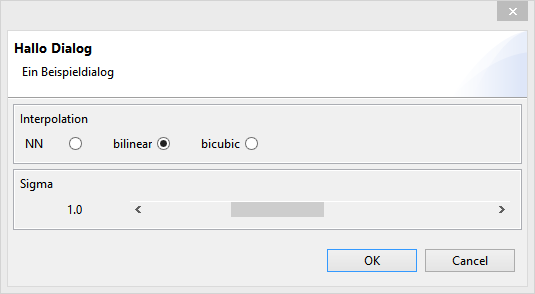
\includegraphics[angle=0,width=8cm]{./img/dialog_example.png}}
   \caption{Die visuelle Darstellung des Dialogs aus Listing \ref{dynamicex}}
  \label{dialog_example}
  \vspace{0.5cm}
\end{figure}

\FloatBarrier
\subsection{Der Laplace-Operator}

Der Laplace-Operator wird zur Schärfung von Bildern eingesetzt und dient als Beispiel für die Umsetzung eines zweidimensionalen Plug-ins. Die \textit{process}-Methode aus Listing \ref{laplace} zeigt eine Implementierung des Filters. Der Parameter \textit{arg0} enthalt die aktuelle Bildschicht des aktiven ImageViews.\\
In Zeile $6$ wird mit Hilfe der einfachen Fabrikfunktion das Bild für die Filterergebnisse erzeugt, da der Bildtyp von \textit{arg0} nicht explizit bekannt ist. In Zeile $16$ wird das Quellbild \textit{arg0} durchlaufen und gefiltert. In Zeile $31$ wird \textit{copySignificantAttributes} aufgerufen. Damit werden essentielle Bildeigenschaften vom Parameterbild in das aufrufende Bild kopiert. Zu den Eigenschaften zählen zum Beispiel \textit{WindowWidth}, \textit{WindowCenter} oder \textit{ImagePosition}.\\
Sind diese Werte vom Anwender im Rückgabewert von \textit{process} nicht gesetzt, werden die Eigenschaften von \textit{arg0} in das Ergebnisbild von jMediKit kopiert. Damit wird eine korrekte Anzeige im ImageView garantiert.\\
Nach der Rückgabe des geschärften Bildes, wird es von der Anwendung angezeigt.

\begin{figure*}[htb]
%\subfigure[Keypoints]{\includegraphics[width=0.49\textwidth]{./img/basmati_keypoints.png}}\hfill
\centering
\fbox{
\subfigure[Anzeige des ungefilterten Bildes im \textit{ImageViewComposite}]{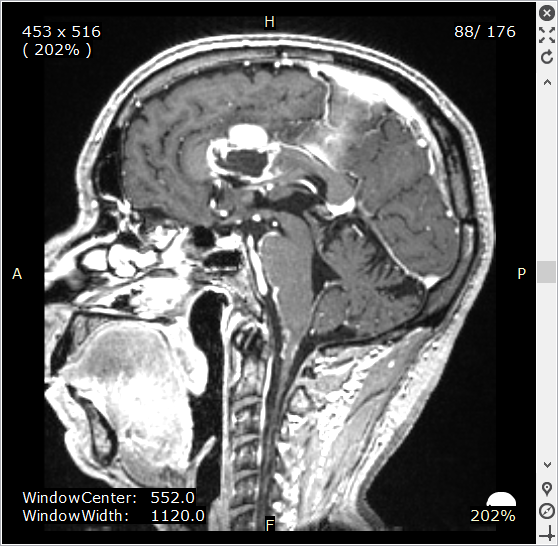
\includegraphics[width=0.48\textwidth]{./img/laplace.png} \label{laplace:unfiltered}}
\subfigure[Anzeige des Bildes, nachdem der Laplace-Operator angewendet wurde]{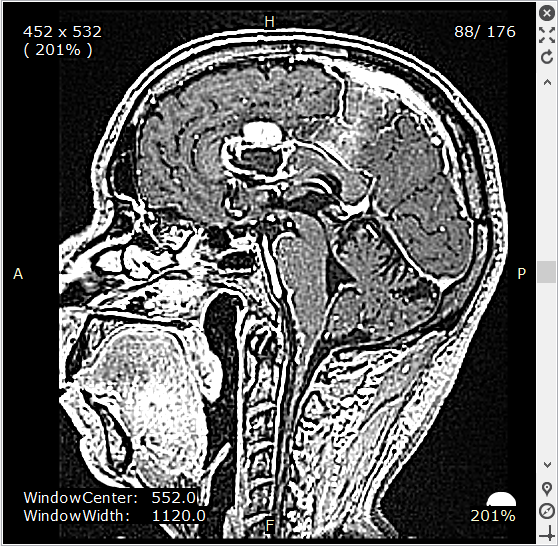
\includegraphics[width=0.48\textwidth]{./img/laplace_filtered.png} \label{laplace:filtered}}
}
\caption{Filterung eines medizinischen Bildes mit dem Laplace-Operator}
\label{laplace_filter}
\end{figure*}

\lstset{
language=Java,
caption={Implementierung der process-Methode des Laplace-Operators},
label=laplace,
xleftmargin=1em,
xrightmargin=1em,
numbers=left,
backgroundcolor=\color{lgrey},
}  
\begin{figure}[htbp]
\begin{lstlisting}[frame=leftline]
@Override
public AImage process(AImage arg0) {
  int width = arg0.getWidth();
  int height = arg0.getHeight();
  //AImage zur Speicherung des Ergebnisses	
  AImage edgeImg = SimpleImageFactory.getAbstractImage(arg0.getImageType(), width, height);

  int[][] filter = new int[3][3];
  filter[0][0] = 1; filter[0][1] = 2;   filter[0][2] = 1; 
  filter[1][0] = 2; filter[1][1] = -12; filter[1][2] = 2;
  filter[2][0] = 1; filter[2][1] = 2;   filter[2][2] = 1;

  int fw = filter.length/2;
  
  //ueber alle Pixel		
  for(int y = 1; y < height-1; y++){
    for(int x = 1; x < width-1; x++){
      int sum = 0;
      //Filterung
      for(int j = -fw; j <= fw; j++){
        for(int i = -fw; i <= fw; i++){
          int value = arg0.getPixel(x+i, y+j);
          int filter_value = filter[j+fw][i+fw];
          sum = sum + value*filter_value;
        }
      }
      //setzen des Ergebniswertes
      edgeImg.setPixel(x, y, sum);
    }
  }
  edgeImg.copySignificantAttributes(arg0);
		
  AImage img = SimpleImageFactory.getAbstractImage(arg0.getImageType(), width, height);
		
  //Differenzbild img = arg0 - edgeImg berechnen
  return img;
}
\end{lstlisting}
\end{figure}
 
\FloatBarrier
\subsection{Der Sobel-Operator}

Der Sobel-Operator dient als Kantendetektor zur Visualisierung harter Intensitätsübergänge in Bildern. Listing \ref{sobel} zeigt die Implementierung von \textit{process}\footnote{Zur Übersichtlichkeit wurde ein Teil des Quelltextes ausgelassen. Der vollständige Code befindet sich auf dem beiliegenden Datenträger.}.

\lstset{
language=Java,
caption={Implementierung der process-Methode des Sobel-Operators},
label=sobel,
xleftmargin=1em,
xrightmargin=1em,
numbers=left,
backgroundcolor=\color{lgrey},
}  
\begin{figure}[htbp]
\begin{lstlisting}[frame=leftline]
@Override
public List<AImage> process(List<AImage> arg0, int arg1) {
		
  //Variablenbelegung
		
  //Filter in x- und y-Richtung
  int[][] x_dir = new int[3][3]; int[][] y_dir = new int[3][3];
  	
  for(int z = 0; z < arg0.size(); z++){

    AImage img = arg0.get(z);
    AImage edgeImg = SimpleImageFactory.getAbstractImage(img.getImageType(), width, height);

    for(int y = 1; y < height-1; y++){
      for(int x = 1; x < width-1; x++){
        for(int j = -1; j <= 1; j++){
          for(int i = -1; i <= 1; i++){
            //Filterung
          }
        }
        //Kantenstaerke
					
        //nach Pruefung auf Ueberschreitung von min und max durch E_xy
        //Pixel setzen
      }
    }
    edge.add(edgeImg);
  }
  return edge;
}
\end{lstlisting}
\end{figure}

Sobel wird im Beispiel als 3D-Plug-in realisiert, wie die Parameter der Methode zeigen. Der wesentliche Unterschied zur Laplace-Implementierung liegt in Zeile $9$, indem der gesamte Bildstapel durchlaufen wird und der Filter auf den Ebenen x, y und z arbeitet.

\begin{figure*}[htb]
%\subfigure[Keypoints]{\includegraphics[width=0.49\textwidth]{./img/basmati_keypoints.png}}\hfill
\centering
\fbox{
\subfigure[Anzeige des ungefilterten Bildes im \textit{ImageViewComposite}]{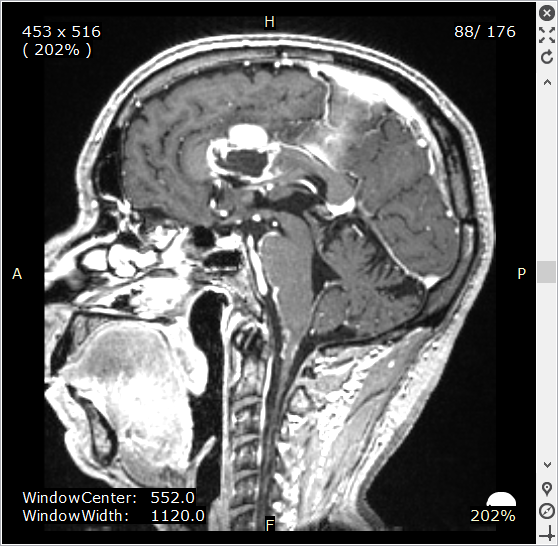
\includegraphics[width=0.48\textwidth]{./img/laplace.png} \label{sobel:unfiltered}}
\subfigure[Anzeige einer Bildschicht, nachdem der Sobel-Operator auf den Bildstapel angewendet wurde]{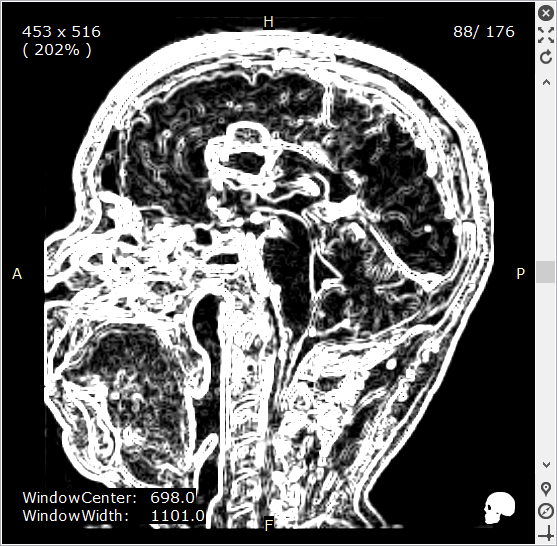
\includegraphics[width=0.48\textwidth]{./img/sobel_filtered.png} \label{sobel:filtered}}
}
\caption{Filterung eines medizinischen Bildes mit dem Sobel-Operator}
\label{sobel_filter}
\end{figure*}

\FloatBarrier
\subsection{Der ConnectedThresholdImageFilter aus dem SimpleITK}

Der ConnectedThresholdImageFilter ist ein Filter aus der SimpleITK-Bibliothek und wird zur Segmentierung von Bildstrukturen eingesetzt. Für eine Anwendung des Filters müssen Saatpunkte mit dem \textit{PointTool} im Bild definiert werden. Anhand dieser Punkte wird mit einem oberen und unteren Schwellwert bestimmt, ob ein Pixel zu der zu segmentierenden Struktur gehört. Die Eingabe der Schwellwerte wird mit Hilfe eines \textit{GenericPlugInDialogs} implementiert(Listing \ref{connopt}).Der Dialog besteht aus den zwei Integerwerten \textit{upperThreshold} und \textit{lowerThreshold}.

\lstset{
language=Java,
caption={Die options-Methode von ConnectedThresholdImageFilter},
label=connopt,
xleftmargin=1em,
xrightmargin=1em,
numbers=left,
backgroundcolor=\color{lgrey},
}  
\begin{figure}[htbp]
\begin{lstlisting}[frame=leftline]
@Override
  protected int options() {
  //Dialog erzeugen
  dialog.addIntegerItem("Lower Threshold", 0);
  dialog.addIntegerItem("Upper Threshold", 0);
  dialog.open();
		
  lowerThreshold = (int) dialog.getItemValue("Lower Threshold");
  upperThreshold = (int) dialog.getItemValue("Upper Threshold");

  return 0;
}
\end{lstlisting}
\end{figure}

Listing \ref{connproc} zeigt die Implementierung des Filters. Die Liste in Zeile $2$ dient zur Speicherung der segmentierten Bilder. Da der ConnectedThresholdImageFilter ein 3D-Plug-in ist, wird in Zeile $4$ der Bildstapel durchlaufen. Folgend werden, falls vorhanden, die Saatpunkte der aktuellen Schicht gelesen(Zeile $5$) und anschließend aus dem Bild ein SimpleITK-Bild erzeugt(Zeile $7$). In Zeile $8$ erfolgt die Instantiierung des Filters selbst. Damit der Filter arbeiten kann, müssen einige Werte gesetzt werden. Die Zeilen $10-12$ legen die Schwellwerte aus dem Dialog fest und es wird ein Wert bestimmt, den zu ersetzende Pixel zugewiesen bekommen. $14-23$ dienen dem Auslesen der Saatpunkte. Jeder definierte Punkt wird dem Filter zugewiesen. Innerhalb des SimpleITK werden die Punkte als \textit{VectorUInt32} repräsentiert. Mit dem zweidimensionalen Vektor werden die Saatpunkte konvertiert. Zeile $23$ führt den Algorithmus mit der \textit{execute}-Methode aus. Nach einer Konvertierung in ein \textit{AImage} in $24$, wird das Ergebnisbild der Liste hinzugefügt. Ist der komplette Bildstapel abgearbeitet, werden die segmentierten Daten im aktiven ImageView angezeigt.

\begin{figure*}[htb]
%\subfigure[Keypoints]{\includegraphics[width=0.49\textwidth]{./img/basmati_keypoints.png}}\hfill
\centering
\fbox{
\subfigure[Anzeige des ungefilterten Bildes im \textit{ImageViewComposite}. Die rot markierten Punkt sind die ausgewählten Saatpunkte.]{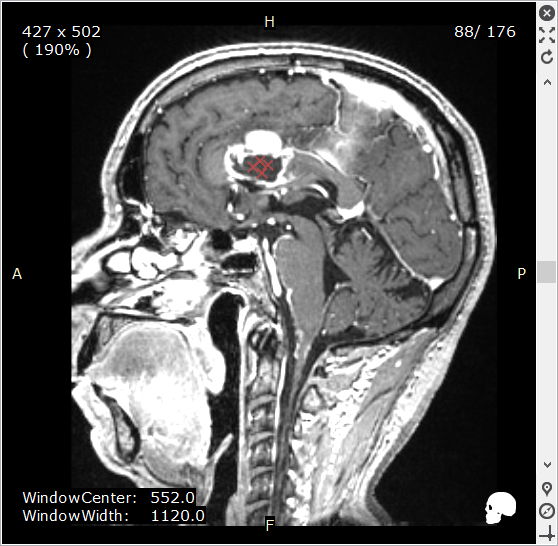
\includegraphics[width=0.41\textwidth]{./img/ctf.png} \label{ctf:unfiltered}}
\subfigure[Anzeige einer Schicht der segmentierten Struktur, nachdem der ConnectedThresholdImageFilter auf den Bildstapel angewendet wurde]{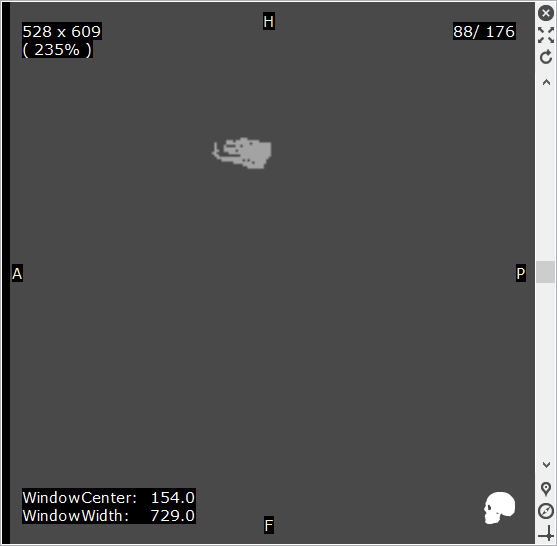
\includegraphics[width=0.41\textwidth]{./img/ctf_filtered.png} \label{ctf:filtered}}
}
\caption{Segmentierung einer Struktur mit dem ConnectedThresholdImageFilter}
\label{ctf_filter}
\end{figure*}

\lstset{
language=Java,
caption={Implementierung der process-Methode des ConnectedThresholdImageFilters},
label=connproc,
xleftmargin=1em,
xrightmargin=1em,
numbers=left,
backgroundcolor=\color{lgrey},
}  
\begin{figure}[htbp]
\begin{lstlisting}[frame=leftline]
@Override
public List<AImage> process(List<AImage> arg0, int arg1) {
  List<AImage> images = new ArrayList<AImage>(arg0.size());
  for(int z = 0; z < arg0.size(); z++){
    ArrayList<Point2D<Float>> selection = arg0.get(arg1).getPoints();
			
    Image source = SimpleITKFactory.getITKImage(arg0.get(z));
    ConnectedThresholdImageFilter segmentationFilter = new ConnectedThresholdImageFilter();
			
    segmentationFilter.setLower(lowerThreshold);
    segmentationFilter.setUpper(upperThreshold);
    segmentationFilter.setReplaceValue((short) 255);
			
    for(Point2D<Float> seed : selection){
      int x = (int) (seed.x*source.getWidth());
      int y = (int) (seed.y*source.getHeight());
				
      VectorUInt32 seed_v = new VectorUInt32(2);
      seed_v.set(0, x);
      seed_v.set(1, y);
				
      segmentationFilter.addSeed(seed_v);
    }
    Image out = segmentationFilter.execute(source);
    images.add(SimpleITKFactory.getAImage(out));
  }
  return images;
}
\end{lstlisting}
\end{figure}

\FloatBarrier
\section{Erweiterung der Anwendungsstruktur mit dem Eclipse Application Model}
Anders als die Plug-ins werden Erweiterungen der Anwendung mit dem Application Model erst nach einem erneuten Buildprozess integriert. Dadurch richtet sich die Kategorie der Modularisierung an Entwickler, die jMediKit gezielt erweitern.\\
Als Beispiel für eine modulare Erweiterung soll im \textit{PartStack} des \textit{DicomBrowsers} ein neuer \textit{Part} hinzugefügt werden, der theoretisch alle verfügbaren PACS im Netzwerk anzeigt. Implementiert wird nur eine minimale Oberfläche.\\
Bevor die Struktur erweitert werden kann, muss entsprechend der Anleitung in Anhang \ref{install_eclipse} die Eclipse-Installation vorbereitet sein. Sind die drei Projekte im \textit{Project Explorer} vorhanden, kann mit der Erweiterung begonnen werden.\\
Im Projekt \textit{org.jmedikit.plugin} befindet sich die Datei \textit{Application.e4xmi}\footnote{Die XML-Datei Application.e4xmi kann auch direkt im Quelltext bearbeitet werden. Die Darstellung in Eclipse erhöht die Benutzerfreundlichkeit zur Anpassung der Werte}. Darin sind alle strukturellen Informationen zu der Anwendungsoberfläche, Menüs, Handler, Com\-mands und die Referenzen auf die implementierenden Klassen hinterlegt. Mit einem Doppelklick kann diese geöffnet werden und es zeigt sich ein Fenster wie in Abbildung \ref{e4xmi}. Die linke Spalte zeigt die Applikationsstruktur und rechts sind die entsprechenden Eigenschaften des gewählten Elements zu sehen. Ab dem Element \textit{Windows} im Strukturbaum werden die Anwendungsteile angezeigt. Dieser Teilbaum entspricht der Abbildung \ref{hierarchy} aus Kapitel \ref{architecture}. Da der \textit{PartStack} in dem der \textit{DicomBrowser} liegt erweitert werden soll, muss bis zu diesem Knoten navigiert werden. Der richtige \textit{PartStack} hat die Id \textit{org.jmedikit.plugin.dicombrowserStack}.
\begin{figure}[H]
  \vspace{0.5cm}
  \centering
  \fbox{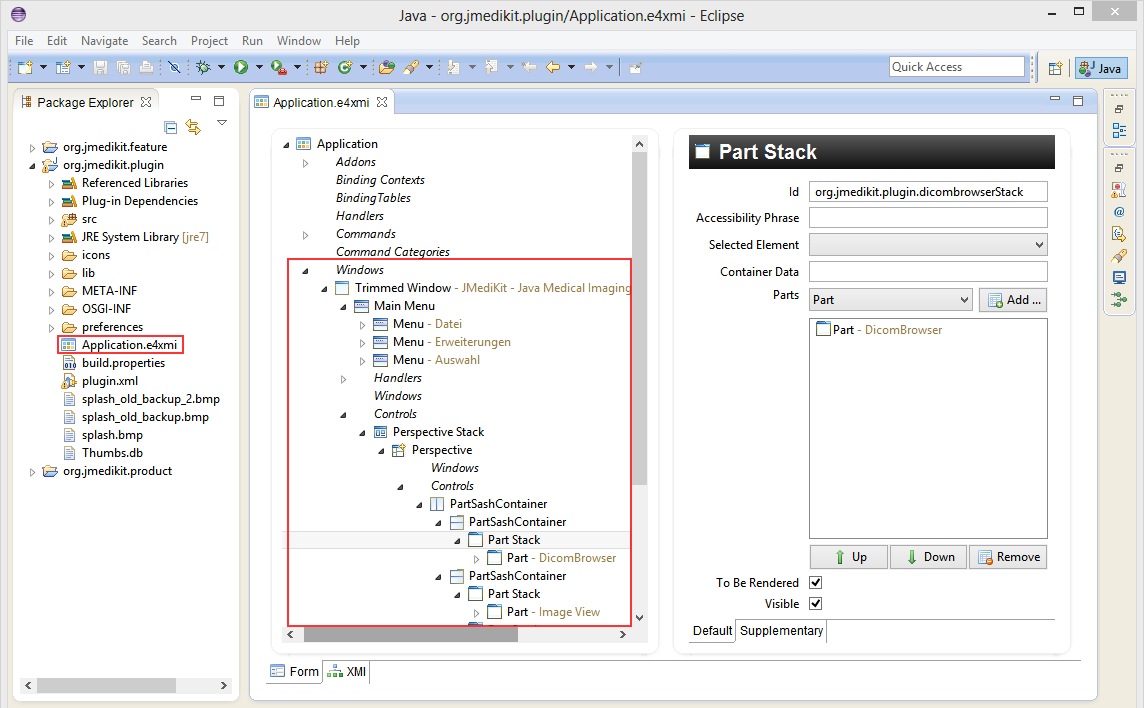
\includegraphics[angle=0,width=\textwidth]{./img/part_exmi.png}}
   \caption{Die Datei Application.e4xmi}
  \label{e4xmi}
  \vspace{0.5cm}
\end{figure}

Nach der Auswahl des \textit{PartStack}-Elements sind rechts dessen Eigenschaften inklusive einer Liste aller enthaltenen \textit{Parts} zu sehen(Abbildung \ref{partadd}). Über das Formularfeld \textit{Parts} kann mit einem Klick auf \textit{Add} ein neuer Kindknoten eingefügt werden. Im diesem Beispiel wird dem Stack ein neuer \textit{Part} untergeordnet.

\begin{figure}[H]
  \vspace{0.5cm}
  \centering
  \fbox{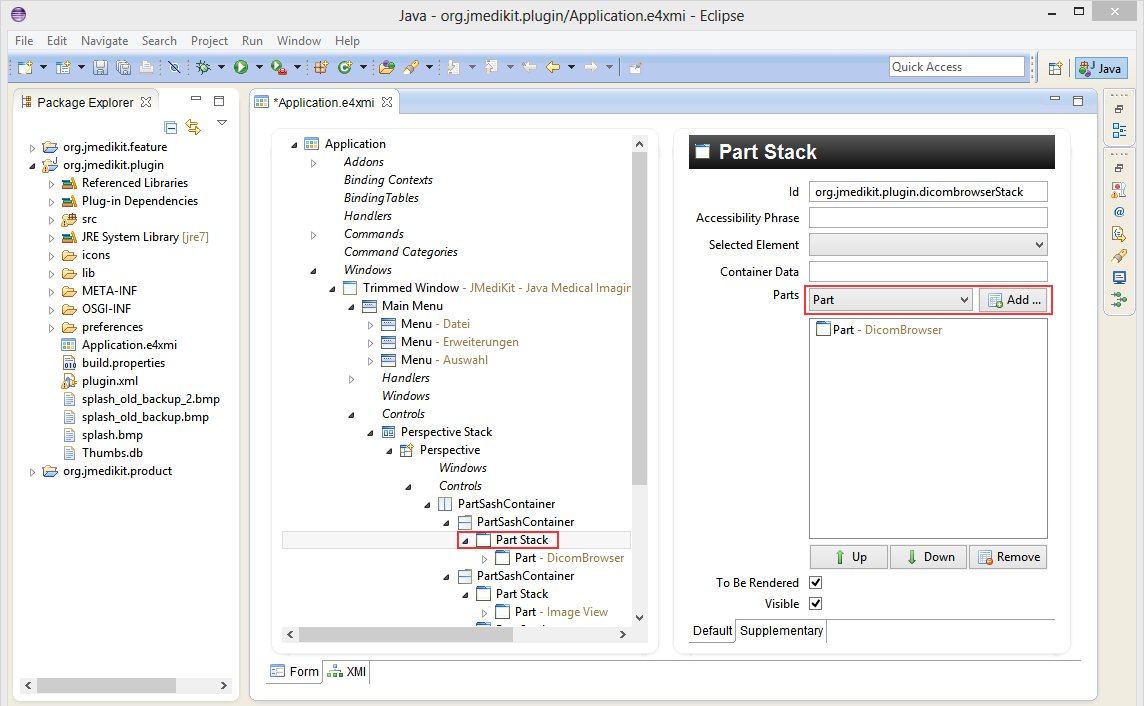
\includegraphics[angle=0,width=\textwidth]{./img/part_add.png}}
   \caption{Einfügen der Part-Struktur}
  \label{partadd}
  \vspace{0.5cm}
\end{figure}

Folgend öffnen sich rechts die Eigenschaften des neu angelegten Parts. Wichtige Einstellungen sind \textit{Id}, \textit{Label} und \textit{ClassURI}. Mit Hilfe der Id kann der Part im Quelltext referenziert werden und das Label ist der sichtbare Titel des \textit{Parts} in der Anwendung. Noch ist keine Klasse für das neue Strukturelement definiert worden. Dies kann mit einem Klick auf \textit{ClassURI} erledigt werden. Soll ein Icon neben dem Titel erscheinen, muss zuvor eine Bilddatei nach der Anleitung in Anhang \ref{importicon} importiert werden\footnote{Grundsätzlich ist es ausreichend, die Bilddateien im \textit{icon}-Ordner zu speichern, aufgrund einer durchgehenden Konsistenz ist es allerdings besser das Bild komplett zu importieren.}.

\begin{figure}[H]
  \vspace{0.5cm}
  \centering
  \fbox{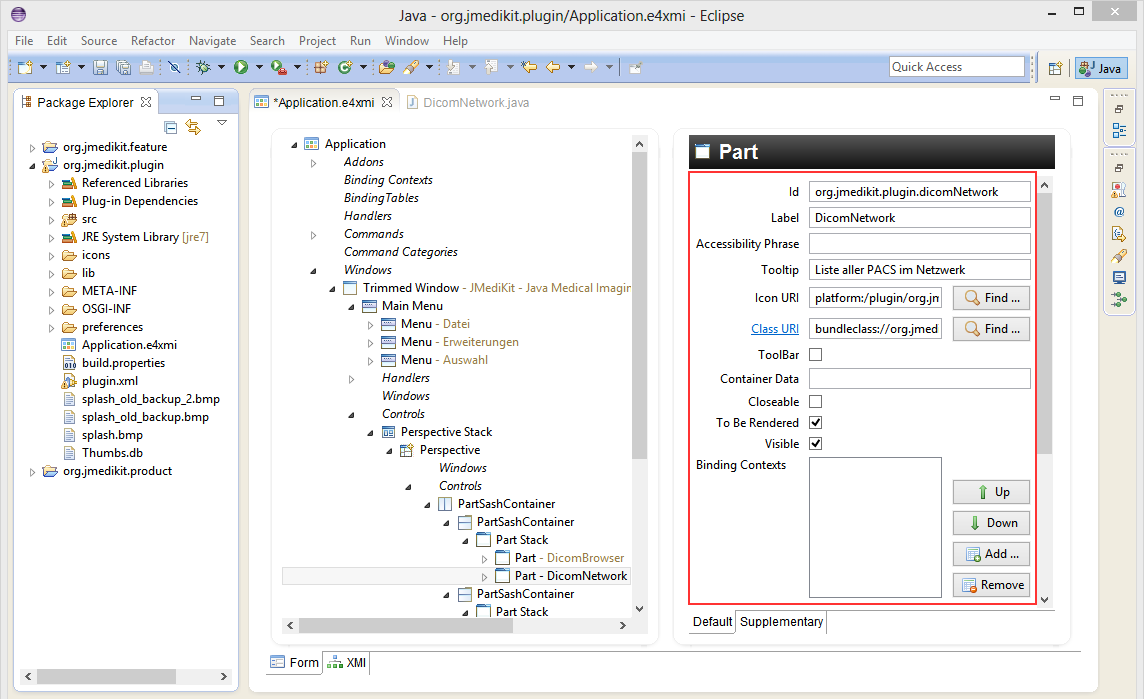
\includegraphics[angle=0,width=\textwidth]{./img/part_part.png}}
   \caption{Eigenschaften der Part-Struktur}
  \label{partpart}
  \vspace{0.5cm}
\end{figure}

Die zu erstellende Klasse repräsentiert neben der Benutzeroberfläche auch die Logik hinter dem \textit{Part}. Abbildung \ref{partclass} zeigt den Dialog zum Erstellen dieser Klasse. Alle \textit{Part}-Implementierungen befinden sich im Package \textit{org.jmedikit.plugin.gui}. Der Name ist frei wählbar. Neben Package und Klassenname kann aus vier vordefinierten Methoden gewählt werden.

\begin{figure}[H]
  \vspace{0.5cm}
  \centering
  \fbox{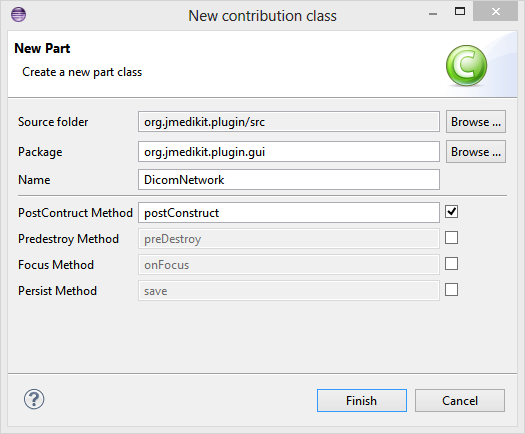
\includegraphics[angle=0,width=0.5\textwidth]{./img/part_class.png}}
   \caption{Erstellen der Klasse}
  \label{partclass}
  \vspace{0.5cm}
\end{figure}

\lstset{
language=Java,
caption={Erweiternder Eintrag einer Konstanten in der Klasse \textit{ImageProvider}},
label=partexample,
xleftmargin=1em,
xrightmargin=1em,
numbers=left,
backgroundcolor=\color{lgrey},
}  
\begin{figure}[htbp]
\begin{lstlisting}[frame=leftline]
public class DicomNetwork {

  @PostConstruct
  public void postConstruct(Composite parent) {
    //definiert das Layout des Elternelements
    //2 Spalten mit gleicher Breite
    GridLayout pGrid = new GridLayout(2, true);
    GridData parentData = new GridData(GridData.FILL_HORIZONTAL);
    parent.setLayout(pGrid);
    parent.setLayoutData(parentData);

    //GUI
    //Suchfeld
    Text search = new Text(parent, SWT.BORDER);
    //Suchbutton
    Button button = new Button(parent, SWT.NONE);
    button.setText("Suche PACS");	
  }	
}
\end{lstlisting}
\end{figure}
Listing \ref{partexample} zeigt eine Beispielimplementierung des \textit{Parts}. Die Annotation \textit{@PostConstruct} sorgt dafür, dass die Methode automatisch nach dem Instantiieren des Objekts ausgelöst wird. Diese enthält als Paramter ein \textit{Composite} und stellt den Einhängepunkt für die weitere Benutzeroberfläche dar.\\
Abbildung \ref{partfinal} zeigt den neuen \textit{Part} in der linken Spalte der Anwendung. Damit wurde dem \textit{PartStack} in dem der \textit{DicomBrowser} enthalten ist das neue \textit{DicomNetwork} eingefügt.

\begin{figure}[H]
  \vspace{0.5cm}
  \centering
  \fbox{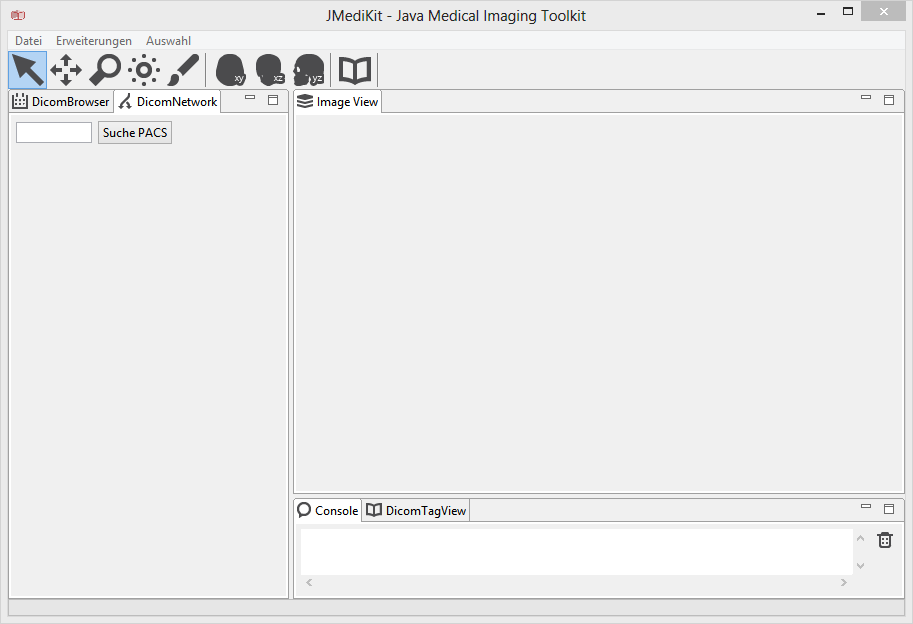
\includegraphics[angle=0,width=\textwidth]{./img/part_final.png}}
   \caption{Anzeige des Parts im PartStack}
  \label{partfinal}
  \vspace{0.5cm}
\end{figure}

\section{Erweiterung der Werkzeuge} \label{roitool}
Neben der Möglichkeit die Anwendungsstruktur zur erweitern und anzupassen, besitzen auch die Werkzeuge von jMediKit den modularen Charakter.
Im folgenden Abschnitt wird der Werkzeugleiste ein weiteres Tool hinzugefügt. Ähnlich dem \textit{PointTool} sollen Bildbereiche ausgewählt werden. Der Unterschied besteht darin, dass keine Punkte bestimmt werden, sondert ein rechteckiger Bildbereich als \textit{Region Of Interest}(ROI) markiert werden kann. Damit werden die Selektionswerkzeuge um das \textit{ROITool erweitert}.\\

\subsection{Hinzufügen eines Menüpunktes} 
Das Menü selbst befindet sich im Applikationsbaum \textit{Window} unter dem Element \textit{TrimBars} $\rightarrow$ \textit{WindowTrim - Top} $\rightarrow$ \textit{ToolBar} und enthält \textit{HandledToolItems}-Strukturen des Application Models als Menüpunkte (Abbildung \ref{toolmenu}). Das bedeutet, dass zu jedem Eintrag ein \textit{Command} mit dem zugehörigen \textit{Handler} erstellt werden muss.

\begin{figure}[H]
  \vspace{0.5cm}
  \centering
  \fbox{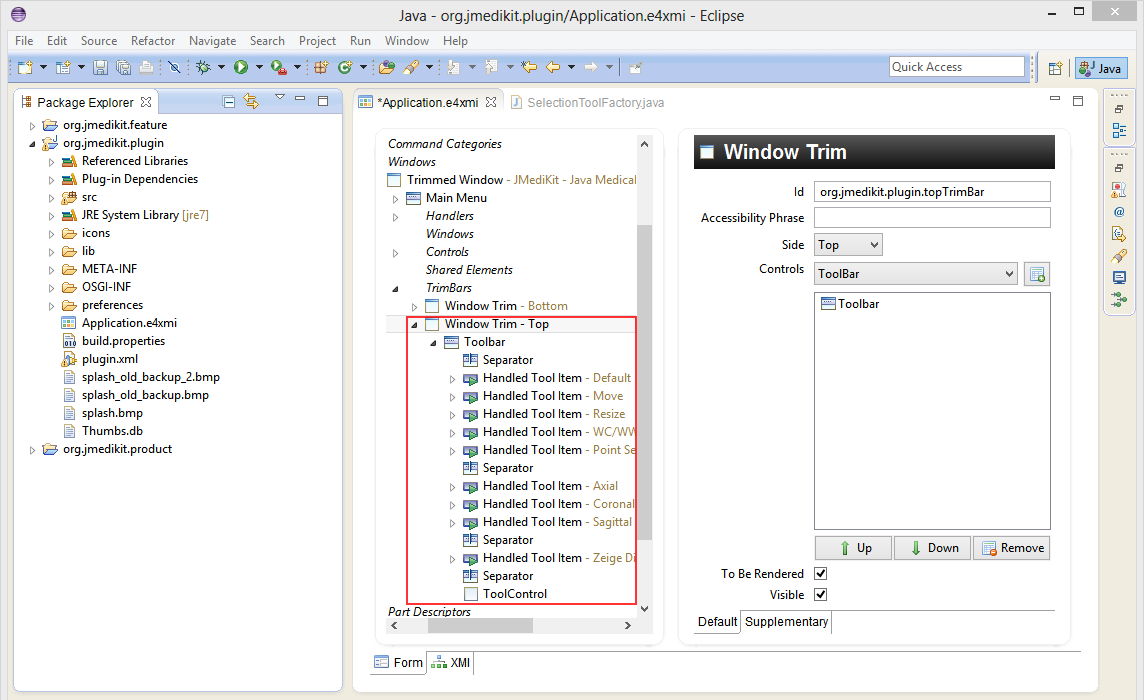
\includegraphics[angle=0,width=\textwidth]{./img/tool_menu.png}}
   \caption{Die Werkzeugleiste im Application Model}
  \label{toolmenu}
  \vspace{0.5cm}
\end{figure}

Die \textit{Commands} sind im Strukturbaum direkt unter \textit{Application} zu finden. Wird das Element ausgewählt, erscheint auf der rechten Seite eine Liste bisher verfügbarer \textit{Commands}. Mit einem Klick auf \textit{Add} kann ein neuer hinzugefügt werden. In den nun angezeigten Einstellungen bekommt die \textit{Id} den Wert \textit{org.jmedikit.plugin.command.toolRoi} und als \textit{Name} wird \textit{toolRoi} eingetragen.\\
Die Implementierung der Befehle finden in den \textit{Handlern} statt. Diese sind im Baum unter \textit{Window} angesiedelt. Nach der Auswahl erscheint die Liste der erstellten \textit{Handler}. Wie schon bei den \textit{Commands}, wird ein neuer \textit{Handler} hinzugefügt und \textit{Id} sowie \textit{Name} vergeben. Unter dem Punkt \textit{Command} wird der zuvor erstellte Befehl angegeben. Mit einem Klick auf \textit{ClassURI}, wie in Abbildung \ref{tool_handlerclass} dargestellt, kann die entsprechende Klasse erstellt werden. Üblicherweise liegen Handlerklassen im Package \textit{org.jmedikit.plugin.gui.handler} und haben den Namen \textit{ToolNameHandler}.

\begin{figure}[H]
  \vspace{0.5cm}
  \centering
  \fbox{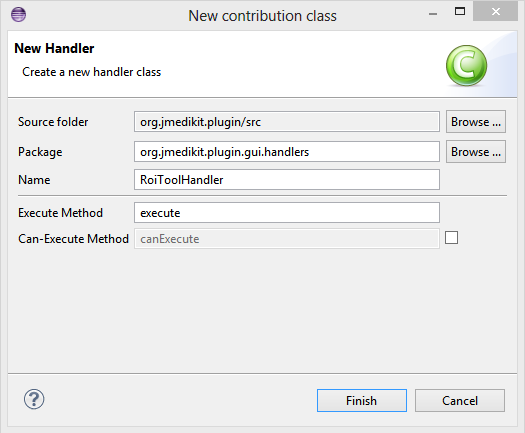
\includegraphics[angle=0,width=0.5\textwidth]{./img/tool_handlerclass.png}}
   \caption{Erstellung einer Klasse für die Handlerimplementierung}
  \label{tool_handlerclass}
  \vspace{0.5cm}
\end{figure}

Im nächsten Schritt erfolgt das Hinzufügen eines \textit{HandledToolItem} zu dem Element unter \textit{Window} $\rightarrow$ \textit{TrimBars} $\rightarrow$ \textit{WindowTrim - Top} $\rightarrow$ \textit{ToolBar}. Die Reihenfolge der Liste entspricht der Darstellung in der Anwendung. Unter den Einstellungen muss \textit{Id}, \textit{Label} und \textit{Command} mit Werten belegt werden. Als \textit{Type} muss die Option \textit{Radio} gewählt werden, da genau ein Werkzeug aktiv ausgewählt sein darf. Unter dem Punkt \textit{IconURI} wird bei Bedarf ein Bild angegeben. Abbildung \ref{tool_handleditem} zeigt die gesetzten Einstellungen und \ref{tool_menunew} die neue Werkzeugleiste mit dem \textit{ROITool} als erweiterten Eintrag.

\begin{figure}[H]
  \vspace{0.5cm}
  \centering
  \fbox{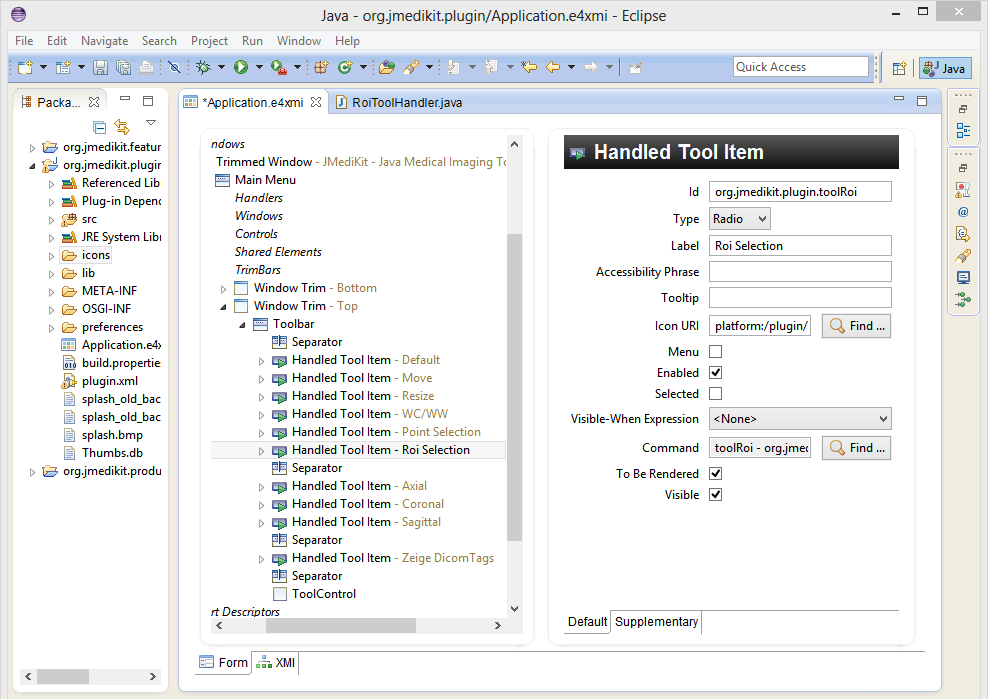
\includegraphics[angle=0,width=0.8\textwidth]{./img/tool_handleditem.png}}
   \caption{Einstellungen des neuen Menüpunktes}
  \label{tool_handleditem}
  \vspace{0.5cm}
\end{figure}


\begin{figure}[H]
  \vspace{0.5cm}
  \centering
  \fbox{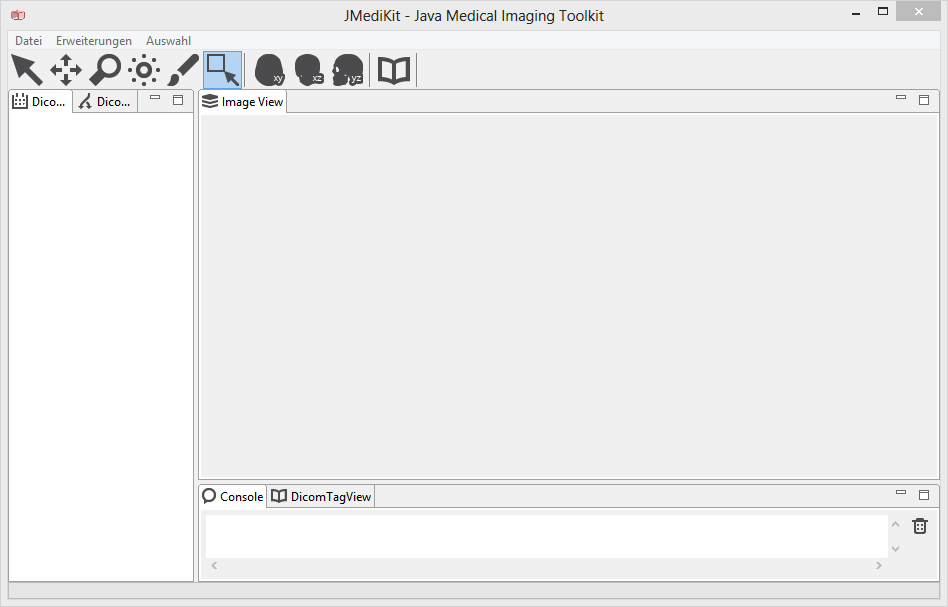
\includegraphics[angle=0,width=0.8\textwidth]{./img/tool_menunew.png}}
   \caption{Anzeige der erweiterten Werkzeugleiste}
  \label{tool_menunew}
  \vspace{0.5cm}
\end{figure}

\subsection{Hinzufügen der Funktionalität}

Nach der Erweiterung der Werkzeugleiste kann die grundlegende Klasse des Werkzeugs erstellt werden. Wichtig ist die Generalisierung von \textit{ATool}, wie in Listing \ref{toolclass} zu sehen ist.

\lstset{
language=Java,
caption={Erweiterung des Basiswerkzeugs},
label=toolclass,
xleftmargin=1em,
xrightmargin=1em,
numbers=left,
backgroundcolor=\color{lgrey},
}  
\begin{figure}[htbp]
\begin{lstlisting}[frame=leftline]
public class RoiTool extends ATool{

  public RoiTool(DicomCanvas c) {
    super(c);
    System.out.println("Hello ROITool");
  }
  
  //weitere Implementierungen abstrakter Methoden
  //der Klasse ATool
}
\end{lstlisting}
\end{figure}

Wird der Menüpunkt in der Werkzeugleiste betätigt, werden Events ausgelöst. In der Klasse \textit{EventConstants} sind diese jeweils in Gruppen definiert. Die Wurzel einer Gruppe hat die in Listing \ref{groups} dargestellte Struktur. \textit{TOOL\_CHANGED} ist der Gruppenname der Events, die Werkzeuge betreffen. Der Zusatz \textit{/*} symbolisiert die Wurzel. Ein spezifisches Werkzeug hat die Form \textit{TOOL\_CHANGED/TOOLNAME}. Durch die Gruppenmechanik ist es möglich, dass eine spezielle Funktion auf alle Werkzeug-Events lauscht und abhängig vom Event die Aufgaben delegiert.

\lstset{
language=Java,
caption={Eventkonstanten der Klasse EventConstants},
label=groups,
xleftmargin=1em,
xrightmargin=1em,
numbers=left,
backgroundcolor=\color{lgrey},
}  
\begin{figure}[htbp]
\begin{lstlisting}[frame=leftline]
public final static String TOOL_CHANGED_ALL = "TOOL_CHANGED/*";
public final static String TOOL_CHANGED_ALL = "TOOL_CHANGED/POINT";
public final static String TOOL_CHANGED_ALL = "TOOL_CHANGED/ROI";
\end{lstlisting}
\end{figure}

Nachdem die Tool-Klasse und das Event kreiert wurden, kann das neue Werkzeug der Fabrik, die für die Erzeugung der Objekte zuständig ist, bekannt gemacht werden. Da das \textit{ROITool} zum Bereich der Selektion gehört, wird die Klasse \textit{SelectionToolFactory} angepasst. In Listing \ref{factory} werden die Modifikationen dargestellt. Innerhalb der Fabrik werden die zugehörigen Events in einer Konstante gespeichert. Die Methode \textit{produce} regelt die Objekterzeugung. Klickt der Anwender auf den Menüpunkt \textit{ROITool} wird das Event ausgelöst und der Werkzeugname an die Fabrik übergeben. Aufgrund des \textit{toolname} wird das richtige Werkzeug erstellt.

\lstset{
language=Java,
caption={Modifikation der SelectionToolFactory},
label=factory,
xleftmargin=1em,
xrightmargin=1em,
numbers=left,
backgroundcolor=\color{lgrey},
}  
\begin{figure}[htbp]
\begin{lstlisting}[frame=leftline]

public final static String ROI_TOOL = 
  EventConstants.TOOL_CHANGED_ROI;
//weitere Konstanten

@Override
protected ATool produce(String toolname, DicomCanvas c) {
  //Pruefung vorheriger Werkzeuge
  else if(toolname.equals(ROI_TOOL)){
    return new RoiTool(c);
  }
  //Pruefung folgender Werkzeuge
  //Werkzeug wurde nicht gefunden
  else throw new IllegalArgumentException("ERROR");
}
\end{lstlisting}
\end{figure}

Im aktuellen Zustand reagiert das Werkzeug und der neue Menüpunkt noch nicht auf die Eingaben des Benutzers. Es fehlt die Implementierung des \textit{Handlers} und die Kommunikation mit dem \textit{ImageView}. Listing \ref{roihandler} zeigt die Umsetzung der Klasse \textit{ToolRoiHandler}. Das Interface \textit{IEventBroker} regelt die Kommunikation unter den \textit{Parts}. Die Annotation \textit{@Execute} bedeutet, dass die Methode automatisch aufgerufen wird, sobald der Menüpunkt betätigt wird. Sowohl \textit{@Inject} als auch \textit{@Execute} sind Teile des \textit{Dependency Injection Frameworks} von Eclipse. Ein umfassender Artikel ist unter \cite{vogel:di} zu finden.\\
In der Methode \textit{execute} wird dem Werkzeug entsprechend die Fabrik instantiiert. Die Variable \textit{tool} enthält das auszulösende Event. Mit Hilfe des \textit{eventBroker} wird die Benutzereingabe an die lauschenden Methoden der Applikation geleitet. Die Methode \textit{post} erwartet die Event-Konstante und ein ToolEvent, welches die erzeugte Fabrik und den Werkzeugtyp als Parameter erhält.

\lstset{
language=Java,
caption={Implementierung des ToolRoiHandler},
label=roihandler,
xleftmargin=1em,
xrightmargin=1em,
numbers=left,
backgroundcolor=\color{lgrey},
}  
\begin{figure}[htbp]
\begin{lstlisting}[frame=leftline]
@Inject
IEventBroker eventBroker;

@Execute
public void execute() {

  AToolFactory factory = new SelectionToolFactory();
  String tool = EventConstants.TOOL_CHANGED_ROI;

  eventBroker.post(EventConstants.TOOL_CHANGED_ROI, new SelectionToolEvent(factory, tool));
}
\end{lstlisting}
\end{figure}

Klickt der Benutzer auf den Menüpunkt nachdem der \textit{Handler} implementiert wurde, erfolgt die Ausgabe \glqq Hello ROITool\grqq\ auf der Standardausgabe. Das bedeutet, das Werkzeug wurde korrekt erzeugt und kann verwendet werden. Der nächste Schritt ist die Implementierung der Logik.

\subsection{Hinzufügen der Werkzeuglogik}

Ziel des \textit{ROITools} ist es, beliebige rechteckige Flächen innerhalb des Bildes zu markieren, um diese später in Plug-ins benutzen zu können. So können Algorithmen auf ausgewählten Bildbereichen angewendet werden. Folgende Events werden von dem neuen Werkzeug behandelt:

\begin{itemize}
\item \textbf{MouseMove} \\
Bei jeder Mausbewegung wird geprüft, ob eine Maustaste gedrück wird. Ist dies der Fall, wird die Startposition und die Aktuelle Position solange in Datenelementen der Klasse gespeichert, bis die Taste gelöst wird.
\item \textbf{MouseDown} \\
Wird die Maustaste betätigt, werden die Koordinaten auf $0$ zurückgesetzt, damit eine neue Berechnung beginnen kann. Ohne Zurücksetzung wird die zuletzt markierte ROI nochmal auf die Zeichenfläche gemalt und bleibt bis zur ersten Mausbewegung sichtbar.
\item \textbf{MouseUp} \\
 Befindet sich nach dem Loslassen der Maustaste der Start- und Endpunkt des Cursors innerhalb des Bildes, wird eine \textit{Region Of Interest} berechnet. Dazu werden zuerst die Bildkoordinaten der beiden Punkte ermittelt. Darauf folgt eine Normalisierung der Koordinaten und ein Eintrag der im Anschluss erzeugten ROI im Bild.

\pagebreak
\item \textbf{PostCalculation} \\
Nach der Werteberechnung wird das Rechteck der potentiellen ROI auf der Zeichenfläche dargestellt.
\end{itemize}


Ist die Logik implementiert, kann das Werkzeug in vollem Umfang eingesetzt werden. Das Erstellen von Transformationstypen erfolgt analog zu den Selektionswerkzeugen. Eine erweiterte Implementierung des \textit{ROITools} könnte zum Beispiel eine dynamische Größenanpassung der Fläche mit dem Mausrad realisieren.
%Nachdem dem Erstellen des Menüeintrags kann die Fabrik, die für die Erzeugung der Werkzeuge verantwortlich %ist, erweitert werden.